%%%%%%%%%%%%%%%%%%%%%%%%%%%%%%%%%%%%%%%%%%%%%%%%%%%%%%%%%%%%
%%%%%%%%%%%%%%%%%%%%%%%%%%%%%%%%%%%%%%%%%%%%%%%%%%%%%%%%%%%%
%%%%%%%%%%%%%%%%%%%%%%%%%%%%%%%%%%%%%%%%%%%%%%%%%%%%%%%%%%%%
\section{Introduction}
%%%%%%%%%%%%%%%%%%%%%%%%%%%%%%%%%%%%%%%%%%%%%%%%%%%%%%%%%%%%
%%%%%%%%%%%%%%%%%%%%%%%%%%%%%%%%%%%%%%%%%%%%%%%%%%%%%%%%%%%%
%%%%%%%%%%%%%%%%%%%%%%%%%%%%%%%%%%%%%%%%%%%%%%%%%%%%%%%%%%%%

\subsection{PDELab Aims and Features}

\begin{frame}
\frametitle<presentation>{DUNE PDELab Features}
\begin{itemize}
\item Rapid prototyping: Substantially reduce time to implement
discretizations and solvers for systems of PDEs based on DUNE.
\item Simple things should be simple --- suitable for teaching.
\item Discrete function spaces:
\begin{itemize}
\item Conforming and non-conforming,
\item hp-refinement,
\item general approach to constraints,
\item generic generation of product spaces for systems.
\end{itemize} 
\item Operators based on weighted residual formulation:
\begin{itemize}
\item Linear and nonlinear,
\item stationary and transient,
\item FE and FV schemes requiring at most face-neighbors.
\end{itemize} 
\item Exchangeable linear algebra backend. 
\item User only involved with ``local'' view on (reference) element.
\end{itemize}
\end{frame}

\begin{frame}
\frametitle<presentation>{DUNE Module Architecture}
Major DUNE modules are:
\begin{center}
\mode<presentation>{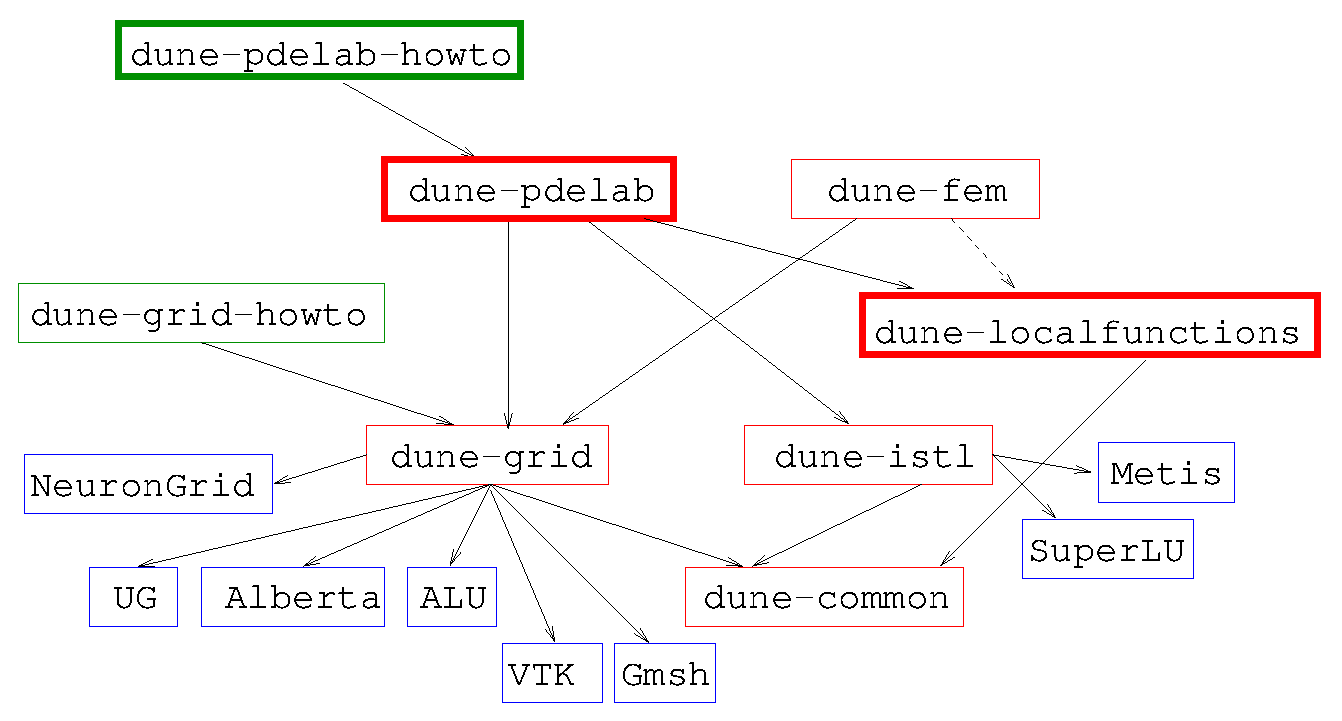
\includegraphics[width=1.0\textwidth]{./EPS/modules}}
\mode<article>{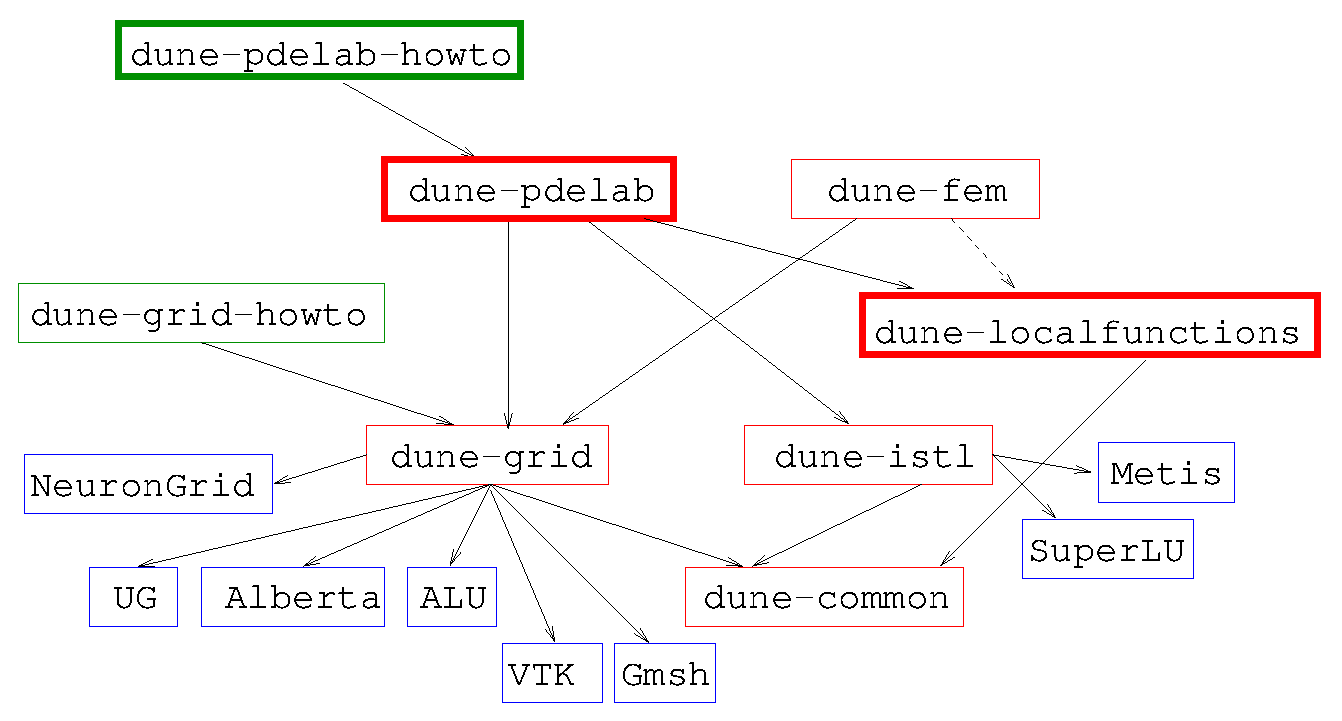
\includegraphics[width=0.7\textwidth]{./EPS/modules}}
\end{center}
\end{frame}

\begin{frame}
\frametitle<presentation>{Required Modules}
To work through the examples the following DUNE modules are required: 
\begin{itemize}
\item \lstinline{dune-common},
\item \lstinline{dune-grid},
\item \lstinline{dune-istl},
\item \lstinline{dune-localfunctions},
\item \lstinline{dune-pdelab},
\item \lstinline{dune-pdelab-howto},
\end{itemize}

In addition, at least one of the grid managers UG, ALU or Alberta is
required to do the examples on simplex grids. 

Note: This course is based on the 2.1snapshot version. In the current trunk
substantial improvements have been made but the user interface is mostly unchanged.
\end{frame}



\subsection{How to Read this Manual}

The main idea of this howto is to introduce the concepts by working
through a set of increasingly complex examples. We will start by 
solving stationary elliptic problems first without and then with constrained spaces
(Dirichlet boundary conditions). After some excursion to linear algebra backends and 
working with CAD models instationary problems and systems will be treated.

\cleardoublepage
